\documentclass[Main.tex]{subfiles}
\begin{document}
\section{From Dynamics to Spatial Models}
Perhaps the simplest way to model a physical system is to write out the equations of motion associated with each individual agent in the system. This approach has been applied in some cases such as animal herding\cite{Correll2008b} where a relatively small number of agents are involved. 

As one can imagine though, modeling every single micro-level interaction between agents quickly gets out-of-hand for very large systems, being analogous in complexity to the n-body problem in physics. The complications that arise when trying to understand these multi-object systems are thus non-trivial, but all is not lost! The established discipline of statistical physics has been tackling these very issues for decades now. Well understood strategies and tools exist for extracting macro-level properties from systems with micro-level particles numbered in the order of Avogadro's constant, $10^{26}$.

We can leverage these tools from statistical physics for understanding and modeling swarm systems as well, even though the number of agents we typically deal with are many orders of magnitude smaller. The use of spatial modeling for swarm robotics has become increasingly popular in the past few years, as is evident from the work of Hamann\cite{Hamann2008, Hamann2010}, Prorok et al.\cite{Prorok2011}, Milutinovi\`{c} and Lima in\cite{Milutinovi2006}.

The central strategy used in spatial modeling of swarm systems involves the use of the Langevin equation, originally used for describing the Brownian motion of a large particle suspended in a medium of smaller particles, e.g. A pollen grain in oil. The Langevin equation is defined as follows\cite{Reif1965}.
\begin{equation}
	m \frac{d\dot{x}}{dt} = \mathcal{F} + F' - \alpha\dot{x}
\end{equation}
Where $\mathcal{F}$ are the forces exerted on the particle at a macroscopic level, $F'$ are the small micro-level fluctuations whose ensemble average $\left<F'\right> = 0$. The final negative term $\alpha\dot{x}$ accounts for friction forces or viscous drag experienced by the large particle during motion.

\mycomment{Describe the terms of the original Langevin equation here.}


It is important to note that the Langevin equation is any differential equation that describes the temporal and spatial evolution of a subset of the degrees of freedom of a particle, i.e. it is not a single equation but a class of equations that all describe the same phenomenon. The original equation for a Brownian agent did not take into consideration the case where an agent could move due to some internal driving force, as robots do. A derivation from Langevin's original equation to the modified form seen below is available in Hamann's dissertation work\cite{Hamann2010}.
\begin{equation}\label{eq:lan}
\V{R}'(t) = -\V{A}(\V{R}(t),t) + B(\V{R}(t),t)\V{F}(t)
\end{equation}

In Eqn.~\eqref{eq:lan}, $\V{R}(t)$ represents the position of the agent at time-$t$, $\V{A}(\V{R}(t),t)$ is a direction function describing the agent's deterministic motion, while $B(\V{R}(t),t)\V{F}(t)$ describes the agent's random motion based on $\V{F}$, a stochastic process (white noise). $\V{A}$ is commonly referred to as the \emph{drift} term in the equation and $B$, the \emph{diffusion coefficient}. $\V{F}(t)$ is a normalized noise term ($\norm{\V{F}(t) = 1}$) with 0 mean and is uncorrelated in time ($\left<\V{F}(t)\V{F}(t') = \delta(t - t')\right>$). Using constant values for drift and diffusion in 1 spatial dimension, Figure~\ref{fig:lan} shows the movement of a robot (or particle) solved using Eqn.~\eqref{eq:lan}.

\begin{figure}[!ht]
\centering\begin{subfigure}{.5\textwidth}
\centering\includegraphics[width=7cm]{assets/LanNoDrift.png}
\end{subfigure}~
\centering\begin{subfigure}{.5\textwidth}
\centering\includegraphics[width=7cm]{assets/LanDrift.png}
\end{subfigure}
\caption{Left: Solution to Langevin equation for a particle in 1D with $\V{A} = 0$, i.e. no drift. Right: Solution with $\V{A} = 0.1$. In both cases the diffusion coefficient is constant, $B = 0.3$, and $\V{F}$ uses an uncorrelated normal distribution with mean $\left<\V{F}\right> = 0$.}\label{fig:lan}
\end{figure}

\subsection{Fokker-Planck Equation: A Macroscopic Model}
From the Langevin equation used in the previous section, we can derive the Fokker-Planck equation as stated below,
\begin{equation}
\PD{\rho(\V{r},t)} = -\nabla(\V{A}(\V{r},t)\rho(\V{r},t))+\frac{1}{2}Q\nabla^2(B^2(\V{r},t)\rho(\V{r},t))
\end{equation}
\begin{figure}[!ht]
\centering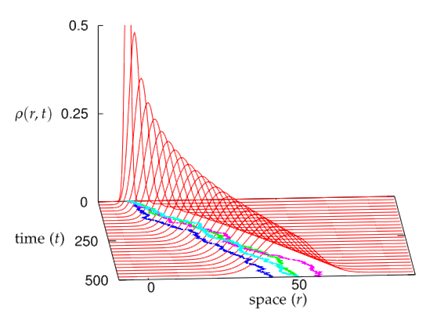
\includegraphics[width=7cm]{assets/fokkerPlanck.png}
\centering\caption{A visual comparison between the spatial micro vs. macro-level equations. The colored lines on the $r$-$t$ plane show the paths taken by individual particles, found via the Langevin equation, while the overarching red curve is the probability distribution for the entire ensemble as described by the Fokker-Planck equation.}\label{fig:fokkerplanck}
\end{figure}

A clear and concise derivation of the above equation from the Langevin equation is provided in section 4.1 of \cite{Hamann2010}, which in turn follows closely from the book \emph{Synergetics} by Haken (1977). The terms $\V{A}$, $B$ and $\V{F}$ reprise their earlier roles from the Langevin equation, while $Q$ is a new displacement term due to collisions between particles. $\rho(\V{r}, t)$ is the probability of encountering a particle at position $\V{r}$ and time $t$. As one can see, the Fokker-Planck equation gives us a \emph{probability distribution} of the positions of particles in space, making it a viable macroscopic model compared to the micro-level Langevin equation which gives us the \emph{position} of a \emph{single} particle in space (see Figure~\ref{fig:fokkerplanck}).

\subsection{Applications}
The Fokker Planck equation is a relatively new tool in the field of swarm robot modeling and has notably been used by Hamann\cite{Hamann2008,Hamann2010}, as well as Prorok, Correll and Martinoli\cite{Prorok2011} in their work on boundary coverage and inspection of jet-turbine engines using swarms of miniature robots. They used a hybrid approach for modeling collective inspection that involves a probabilistic non-spatial model coupled with spatial micro-macro diffusion equations for modeling collective inspection of regular structures to improve consensus with observed experimental values. 

\begin{figure}[!ht]
\centering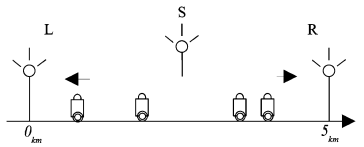
\includegraphics[width=8.5cm]{assets/spatSignal.png}
\centering\caption{Experiment setup for centralized robot population control experiment proposed by Milutinovi\`{c} and Lima in%\cite{Milutinovi2006}
.}\label{fig:signal}
\end{figure}

A spatial model is used in\cite{Milutinovi2006} to control a large scale multi-agent system using centralized controller and three signal sources. The goal of this experiment is to show successful control of a large population of robots by collectively moving them along a 1-dimensional arena using \emph{left}, \emph{right} and \emph{stop} signals from a moving aerial controller. The model accounts for the fact that not all robots receive the signal or change direction/move promptly upon successfully receiving a signal. A visual representation of this setup can be seen in Figure~\ref{fig:signal}.

Although the Fokker-Planck equation is not mentioned explicitly in\cite{Milutinovi2006}, the authors employ the use of a system of PDEs to predict the position of the swarm in the arena via a probability density function (PDF). Their approach is therefore rather similar to the macro-level spatial modeling approach described earlier in this paper. The goal of moving the entire swarm  from point A to point B in a 1D arena just through the use three signals controlled by a centralized controller is formulated as an optimal control problem by the authors. It is solved by introducing appropriate weighting and cost functions to the PDEs and computing the PDF at any given time to predict the collective motion/position of the swarm. The control signals are then switched accordingly to move the swarm in a desired direction. Two particularly insightful plots (Figures 4 \& 5) are provided in\cite{Milutinovi2006} that showcase this result, i.e. the PDF evolution of stopped and moving robot populations as time progresses.

While the non-spatial modeling approaches we have discussed so far use a phenomenological approach to construct the macro-model equations, this is not a viable option in the spatial model case. Typically, the drift and diffusion coefficient functions in the Fokker-Planck equation are adapted based on the swarming task we attempt to model but constructing these functions is not as straightforward as defining the rate equations from a robot controller, as seen in the non-spatial case. The $\V{A}$ and $B$ functions of the Fokker-Planck equation serve to bridge the gap between micro-level and macro-level observations of a swarm system and hence provide quite a challenge to design accurately.
\end{document}